%!TEX root = informe.tex
\chapter{Datos proporcionados por el fabricante}\label{apend:datos}
En este apéndice se incluyen los datos proporcionados por el fabricante acerca del proceso de producción.

\begin{table}[!htb]
\centering
\begin{tabular}{lcccc}
\toprule
\multicolumn{5}{c}{Fórmula base para de adoquín Holanda 6}\\
\midrule
Materia prima & \% Fórmula & Masa (\si{kg}) & Proced. & Dist. (\si{km})\\
\midrule
Árido tipo 5/7 & 37.75 & Alh. Torre & 8\\
Arena tipo 0/5 & 47.16 & Alh. Torre & 8\\
Cemento Portland 52.5N & 10.06 & Málaga-El Palo & 30\\
Agua & 5.03 & 7.54 & Red & -\\
\bottomrule
\end{tabular}
\caption{Fórmula base para de adoquín Holanda 6.}
\label{formulabase}
\end{table}


\begin{figure}[!htb]
\centering
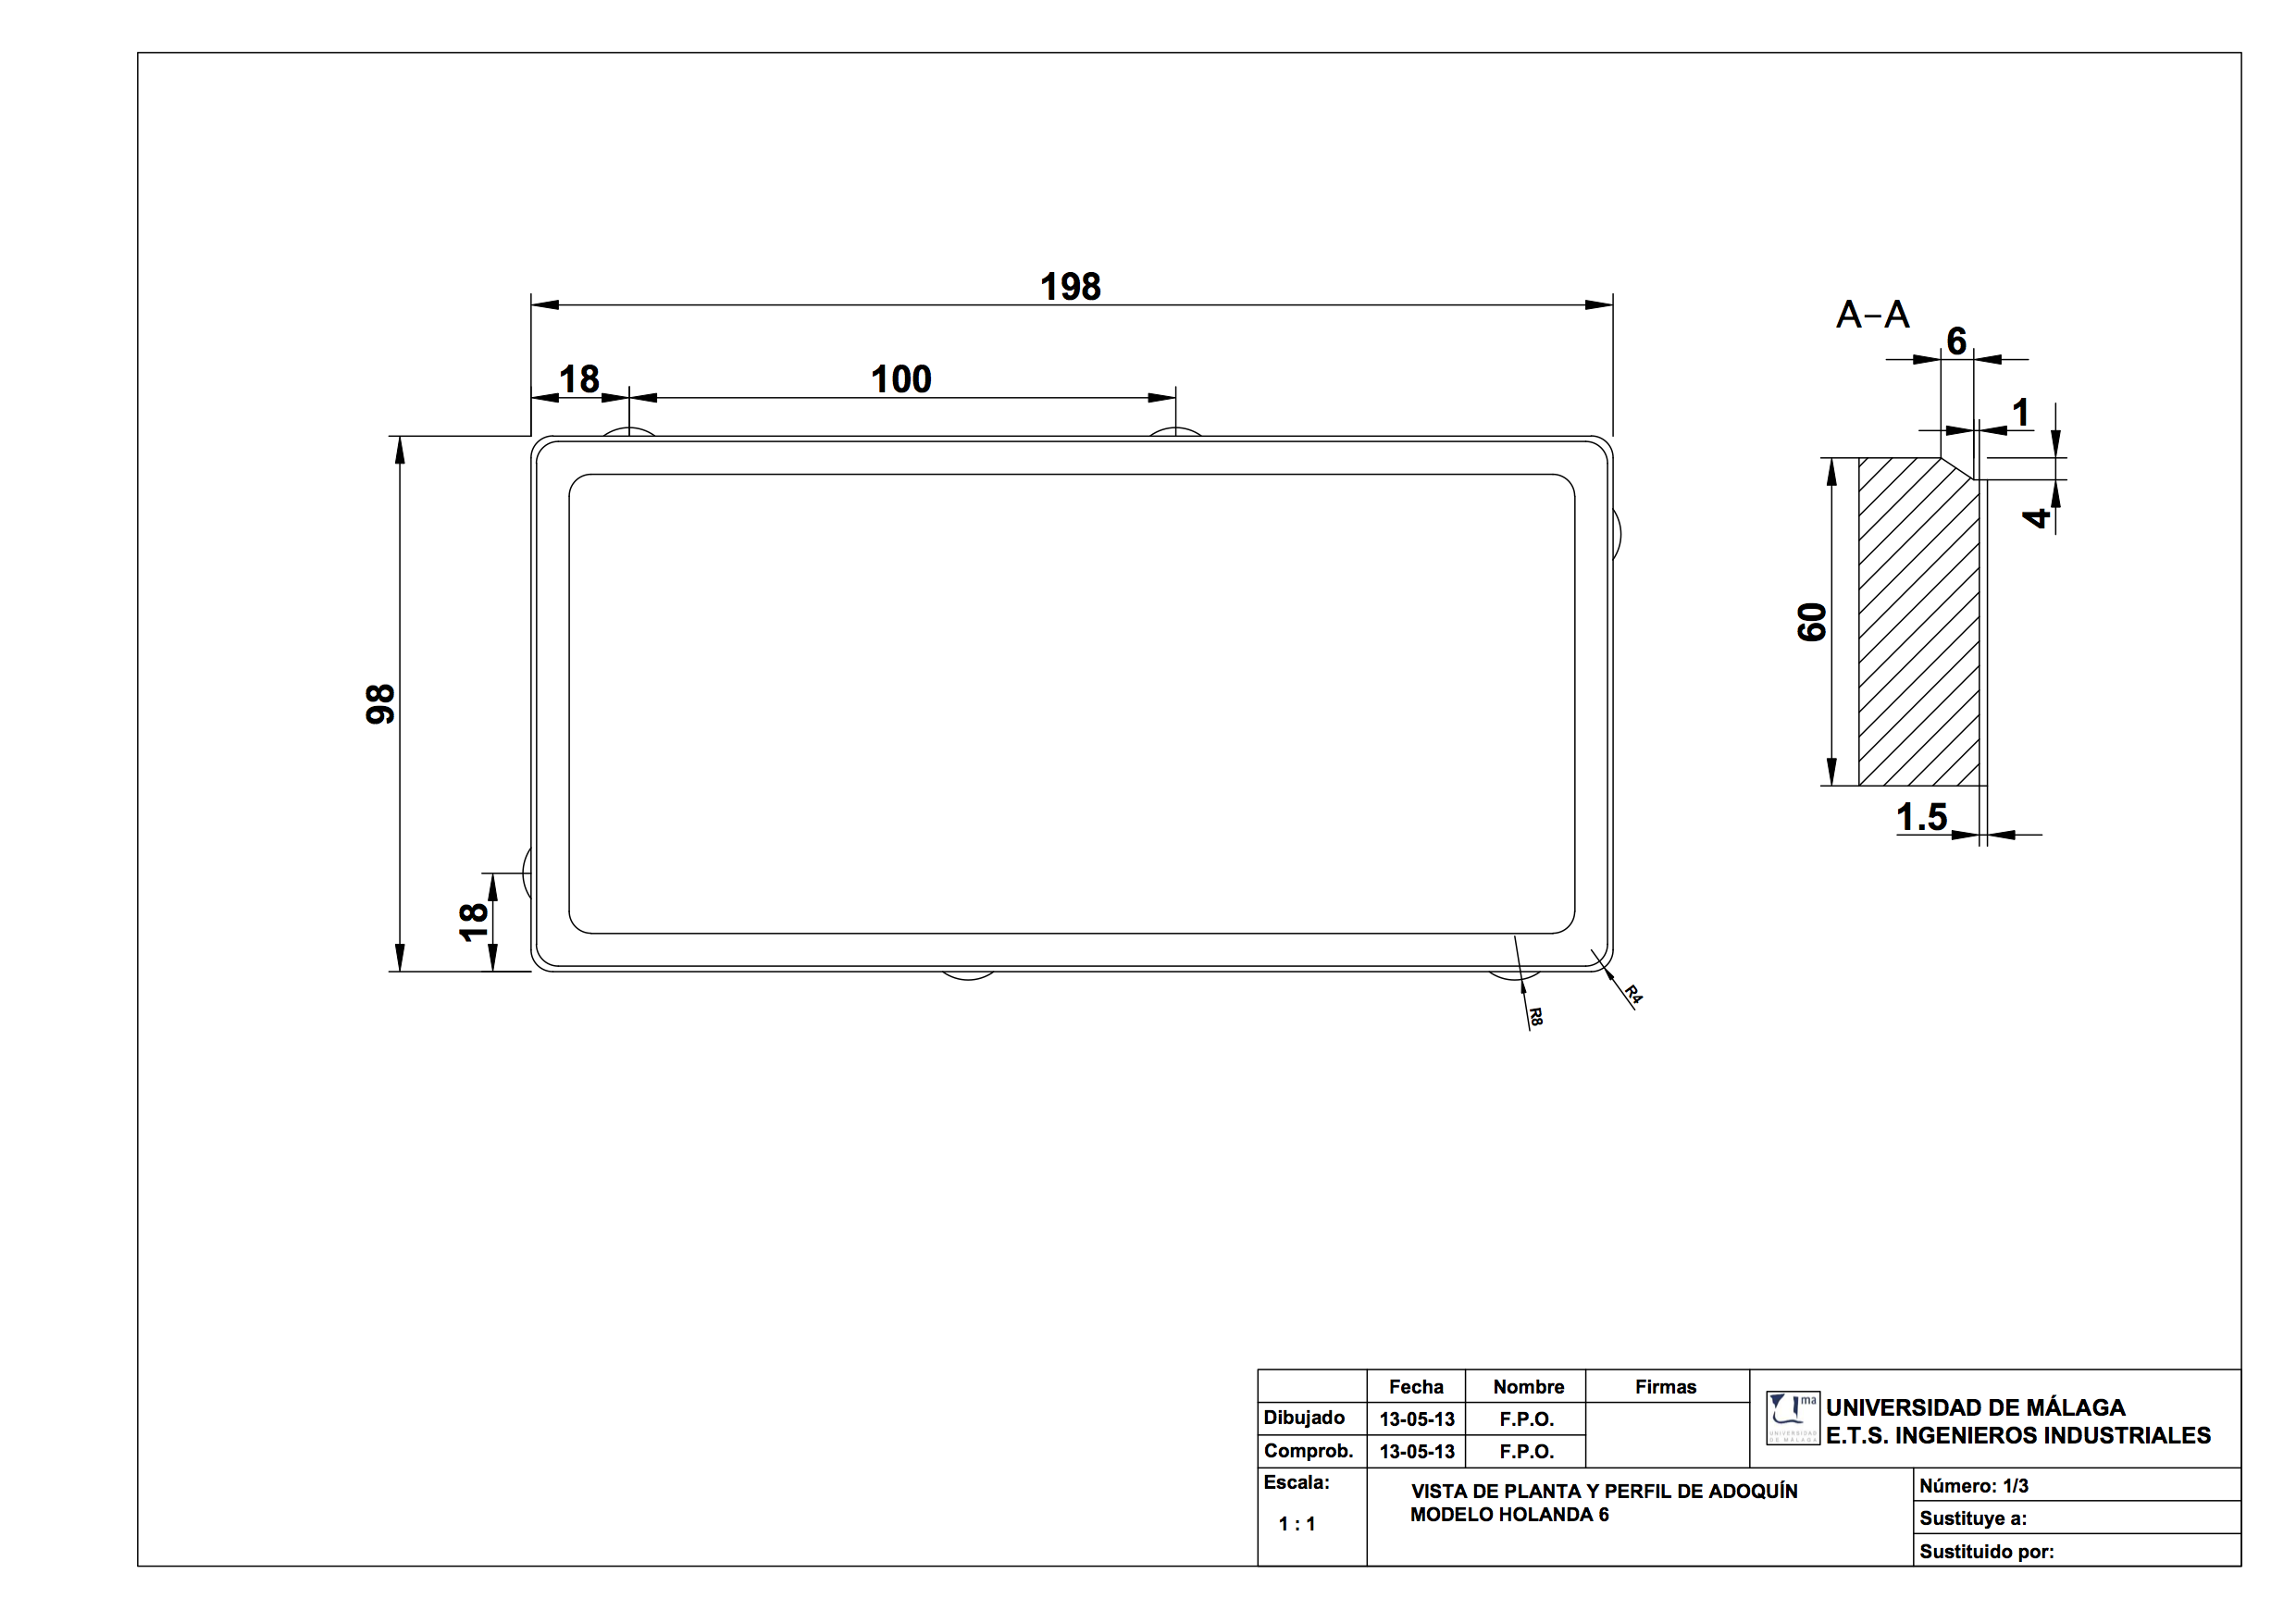
\includegraphics[width=15cm]{plano_adoquin.png}
\caption{Plano modelo adoquín Holanda 6.}
\label{fig:planoadoquin}
\end{figure}

\begin{table}[!htb]
\centering
\begin{tabular}{lcrrr}
\toprule
\multicolumn{5}{c}{Tiempo de proceso y energía por \si{m^2} de adoquín fabricado}\\
\midrule
Proceso & Duración (\si{s}) & Potencia (\si{kW}) & Energía (\si{kJ}) & Energía (\si{MJ})\\
\midrule
Dosif. arena & 3 & 0.7 & 2.1 & 0.0021\\
Dosif. áridos & 3 & 0.7 & 2.1 & 0.0021\\
Cinta transp. arena y áridos  & 21 & 8.7 & 182.7 & 0.1827\\
Cinta transp. cemento  15  6.5 97.5  0.0975\\
Skip  & 27 & 15 & 405 & 0.405\\
Mezcladora & 42 & 31 & 1302 & 1.302\\
Cinta transp. hormigón & 11 & 8 & 88 & 0.088\\
Tolva hormigón 1/2 & 23 & 0.7 & 16.1 & 0.0161\\
Prensado 1/2 & 19 & 23 & 437 & 0.437\\
Cinta transp. piezas frescas 1/2 & 14 & 5.5 & 77 & 0.077\\
Ascensor 1/2 & 1 & 7 & 7 & 0.007\\
Tolva hormigón 2/2 & 23 & 0.7 & 16.1 & 0.0161\\
Prensado 2/2 & 19 & 23 & 437 & 0.437\\
Cinta piezas frescas 2/2 & 14 & 5.5 & 77 & 0.077\\
Ascensor 2/2 & 17 & 7 & 119 & 0.119\\
Multiforca ida & 43 & 12 & 516 & 0.516\\
Multiforca vuelta & 43 & 12 & 516 & 0.516\\
Descensor 1/2 & 17 & 7 & 119 & 0.119\\
Descensor 2/2 & 1 & 7 & 7 & 0.007\\
Transp. bandejas hasta paletiz. & 14 & 1.5 & 21 & 0.021\\
Paletizadora & 10 & 5 & 50 & 0.05\\
Transp. palet & 14 & 1.7 & 23.8 & 0.0238\\
Flejadora & 10 & 1.5 & 15 & 0.015\\
Transp. rodillos hasta recogida  21  1.5 31.5  0.0315\\
Control informatizado 405 1.2 486 0.486\\
Iluminación & 405 & 2.4 & 972 & 0.972\\
\bottomrule
\end{tabular}
\caption{Desglose de procesos y energías del fabricante por \si{m^2} de adoquín fabricado.}
\label{desgloseenergia}
\end{table}
